\pdfoutput=1 % only if pdf/png/jpg images are used
\documentclass{JINST}


\title{New Approaches to Uniform Boosting}

\author{
Aleksandar Bukva$^e$, 
Vladimir Gligorov$^d$,
Alex Rogozhnikov$^{a,b}$\thanks{Corresponding author.}~ ,
Andrey Ustuzhanin$^b$ and
Mike Williams$^c$\\
\llap{$^a$}Lomonosov Moscow State University, Moscow, Russia\\
\llap{$^b$}Yandex LLC, Moscow, Russia\\
\llap{$^c$}Massachusetts Institute of Technology, Cambridge, MA, United States \\
\llap{$^d$}Organisation Europ\'eenne pour la Recherche Nucl\'eaire (CERN), Geneva, Switzerland  \\
\llap{$^e$}Faculty of Physics, Belgrade, Serbia \\
E-mail: \email{alex.rogozhnikov@yandex.ru}}


\abstract{
% Abstract must be short enough to appear in this page together with title, authors, their addresses and keywords.
The use of multivariate classifiers has become commonplace in particle physics. 
Typically, a series of classifiers is trained rather than just one to enhance the performance; this is known as boosting. 

In some applications of high energy physics (i.e., amplitude analyses) 
classifiers should not only optimize some integrated figure of merit, but produce a uniform selection efficiency in a space of selected physical variables.
Recently uBoost technique of boosting was proposed which addresses this issue.

In this paper we introduce several approaches to measure the uniformity of efficiency and propose new boosting techniques.

}





% AMS packages:
\usepackage{amsmath, amsthm, amsfonts}
\usepackage{caption}
\usepackage{subcaption}
\usepackage{float}	


% Theorems
%-----------------------------------------------------------------

\newtheorem{thm}{Theorem}[section]
\newtheorem{cor}[thm]{Corollary}
\newtheorem{lem}[thm]{Lemma}
\newtheorem{prop}[thm]{Proposition}
\theoremstyle{definition}
\newtheorem{defn}[thm]{Definition}
\theoremstyle{remark}
\newtheorem{rem}[thm]{Remark}

\def\RR{\mathbb{R}}
\def\ZZ{\mathbb{Z}}
\newcommand{\abs}[1]{\left\vert#1\right\vert}
\newcommand{\sgn}{\operatorname{sgn}}


%-----------------------------------------------------------------


\begin{document}
\maketitle


\section{Introduction}

Methods of machine learning play an important role in modern particles physics. 
Multivariate classifiers, {\em e.g.}, boosted decision trees (BDTs) and artificial neural networks (ANNs), are now commonly used in analysis selection criteria. BDTs are now even used in software triggers~\cite{ref:lhcbhlt,ref:bbdt}. 
To enhance the performance, a series of classifiers is typically trained; this is a technique known as boosting.
Boosting  involves training many simple classifiers and then building a single composite classifier from their responses.
The classifiers are trained in series with the inputs of each member being augmented based on the performance of its predecessors.  This augmentation is designed such that each new classifier targets more those events which were poorly classified by previous members of the series.  The classifier obtained by combining all members of the series is typically much more powerful than any of the individual members. 

In particle physics, the most common usage of BDTs is in classifying candidates as signal or background.  The BDT is determined by optimizing some figure of merit (FOM), {\em e.g.}, the signal purity or approximate signal significance.  This approach is optimal for a counting experiment; however, in many cases the BDT-based selection obtained in this way is not optimal.  
For example, in a Dalitz-plot (or any angular or amplitude analysis) analysis, obtaining a selection efficiency on signal candidates that is uniform across the Dalitz-plot is more important than any integrated FOM.  Similarly, when measuring a mean particle lifetime, obtaining an efficiency that is uniform in lifetime is what is desired.  In both cases, obtaining a uniform selection efficiency greatly reduces the systematic uncertainties involved in the measurement.  
When searching for a new particle, an analyst may want a uniform efficiency in mass for selecting background candidates so that the BDT-based selection does not generate a fake signal peak.  Furthermore, the analyst may also desire a uniform selection efficiency of signal candidates in mass (or other variates) since the new particle mass is not known.  In such cases, the BDT is often trained on simulated data generated with several values of mass (lifetime, {\em etc.}).  A uniform selection efficiency in mass ensures that the BDT is sensitive to the full range of masses involved in the search. 


\section{Uniformity Measurement}

\section{Measures of uniformity}
In this section we discuss different methods for measuring the uniformity of prediction. 
One typical way of 'checking' uniformity of prediction used by physicists 
is fitting the distribution of the events that were classified as signal (or background) over the 
feature for which you wish to check uniformity.
This approach requires assumptions about the shape of the distribution,
which makes quantitative comparisons of different classifiers difficult.
Our aim here is to explore uniformity figures of merit which make comparing classifiers easier,
analogously to how the area under the ROC curve can be used to compare absolute classifier performance.
%is hardly formalizable, and not automatable --- each time you should assume some kind of distribution. 
%Ideally we want to have some easy-to-use out-of-the-box metrics like FOMs in machine learning (like area under the ROC, f1 or ).

%We start from the simplest case --- when we are fully satisfied by predictions of our classifier. 
The output of event classification is the probability of each event being signal or background,
and it is only after we apply a cut on this probability that events are classified.
An ideal uniformity of signal prediction can then be defined for a given ``uniform feature'' of interest.
It means that whichever cut we select,
the efficiency for a signal event to pass the cut doesn't depend on the uniform feature.
Uniformity for background can be defined in the same manner, but for simplicity,
% (uniform variables) 
%in every region of the uniform variables space the part of signal events that passed the cut is the same.
%In practice, of course, this never happens.
%There is uniformity of predictions on signal and uniformity of efficiency on background, which can be defined one from another by swapping classes. 
in what follows we will only discuss the uniformity of efficiency for signal events.

A trivial example of a classifier that has ideal uniformity is a classifier which returns a random classification probability,
but such a classifier is of course not very useful. One can try to design a uniform classifier with respect to
a given feature by not using this feature, or any correlated features, in the classification; in practice, however,
this approach also tends to lead to poorly performing classifiers. The approach which we take in this paper is 
to explicitly let the classifier learn how to balance non-uniformities coming from different features in such a way
as to generate a classification which is uniform on average. It is then important to be able to accurately measure
the uniformity of classification. 
%What a pity: in practice it's absolutely useless.
% The most significant drawback of the upcoming metrics is they are ill-defined if there are not too many events of the named class. 

Before proceeding, it is useful to define some desirable properties of uniformity metrics
\begin{enumerate}
\item
The metric shouldn't depend strongly on the number of events used to test uniformity;
%(i.e., if we randomly select half of the events, the metrics should roughly be the same)
\item
The metric shouldn't depend on the normalization of the event weights: if we multiply all the weights by some arbitrary number, it shouldn't change at all;
\item 
The metric should depend only on the order of predictions, not the exact values of probabilities.
This is because we care about which events pass the cut and which don't, not about the exact values of predictions.
For example: correlation of prediction and mass doesn't satisfy this restriction.
\item
The metric should be stable against any of its own free parameters: if it uses bins, changing the number of bins shouldn't affect the result,
if it uses $k$-nearest neighbors, it should be stable against different values of $k$.
\end{enumerate}
In what follows we will consider different metrics which satisfy these criteria, and then compare their performance in
some test cases.

\subsection{Standard Deviation of Efficiency on Bins (SDE)}

\def\bineff{\text{eff}_\text{bin}}
\def\binweight{\text{weight}_\text{bin}}
\def\globaleff{\text{eff}}
\def\SDE{\text{SDE}}
\def\bin{\text{bin}}

If the space of uniform features is split into bins, it is possible to define the global efficiency
%  when we select some probability cut, 
%the part of signal events that passes the cut is equal in all bins. Assume we selected some cut, then we have global efficiency
\[
	\globaleff = \dfrac{
		\text{total weight of signal events that passed the cut}}
		{\text{total weight of signal events}},
\]

as well as the efficiency in every bin, 
\[
	\bineff = \dfrac{
		\text{weight of signal events in bin that passed the cut}}
		{\text{weight of signal events in this bin}}.
\]
%So, basically, what we want to have in our dreams:
%\[
%	\bineff = \text{global efficiency} \qquad \forall \; \text{bin}
%\]
One measure of non-uniformity is the standard deviation of bin efficiencies from the global efficiency:
\[
	\sqrt{\sum_{\bin} \left( \bineff - \globaleff \right)^2  }.
\]

%What is bad in this formula that every bin has some impact in the result, which does not depend on how many events are there, so metrics becomes very unstable to deviations in bins with only few events. 
To make the metric more stable against fluctuations in bins which contain very few events, we add weights to the bins (note that $\sum_\bin \binweight = 1$):
\[
	\binweight = \dfrac{\text{total weight of signal events in bin}}
		{\text{total weight of signal events}},
\]
giving the weighted standard deviation (SDE) formula
\[
	\SDE(\globaleff) = 
	\sqrt{\sum_{\bin} \binweight \times \left(\bineff - \globaleff \right)^2}. 
\] 
%In fact, the expression depends on the cut, but for cuts which produce equal efficiency, this is 

%Finally we note that the weighted average of $\bineff$ is $\globaleff$:
%\[
%	\globaleff = < \bineff > =  \sum_{\bin} \binweight \times \bineff,
%\]
%and this is why the introduced metrics was named SDE --- this is a weighted standard deviations of array of bin efficiencies.

%But this is how we measure the non-uniformity for only one fixed cut, 
This formula is valid for any given cut value. To measure the overall non-flatness of the selection, we
take several global efficiencies and use
%(for instance, [0.5, 0.6, 0.7, 0.8, 0.9], because in practice usually we are interested in cuts with high global efficiency) and use 
\[
	\SDE^2  =  \frac{1}{k} 
	\sum_{\globaleff \in [\globaleff_1 \dots \globaleff_k] }  
		\text{SDE}^2(\globaleff)
\]
Another power $p \neq 2$ can be used as well, but $p=2$ is considered as the default value.
%\[
%	\SDE^p(\globaleff) = 
%	\sum_{\bin} \binweight \times \abs{\bineff - \globaleff}^p,
%\qquad
%	\SDE^p  =  \frac{1}{k} 
%	\sum_{\globaleff \in [\globaleff_1 \dots \globaleff_k] }  
%		\text{SDE}^p(\globaleff).
%\]
%
%

\subsection{Theil Index of Efficiency}
\def\theil{\text{Theil}}

The Theil Index is frequently used to measure economic inequality:
\[
	\theil = \frac{1}{N} \sum_i \frac{x_i}{<x>} \ln{\frac{x_i}{<x>}}, 
		\qquad <x> = \frac{1}{N} \sum_i x_i
\]
In our case we have to alter formula a bit to take into account that different bins have different impact, thus the formula turns into
\[
	\theil(\globaleff) = \sum_\bin \binweight \; \frac{\bineff}{\globaleff} \; \ln{\frac{\bineff}{\globaleff}}.
\]
To measure the overall non-flatness, we
average values for several global efficiencies:
\[
	\theil  =  \frac{1}{k} 
	\sum_{\globaleff \in [\globaleff_1 \dots \globaleff_k] }  
		\theil(\globaleff)
\]

\subsection{Distribution Similarity Approach}
\label{sec:similarity}

%Let's start from reformulation of what is uniform predictions in signal. First we split all signal events into some bins in uniform variables. There is some empirical distribution $F_\bin$ of predictions in each bin. 
\begin{figure}[h]
		\centering
		\begin{subfigure}[b]{0.8\textwidth}
			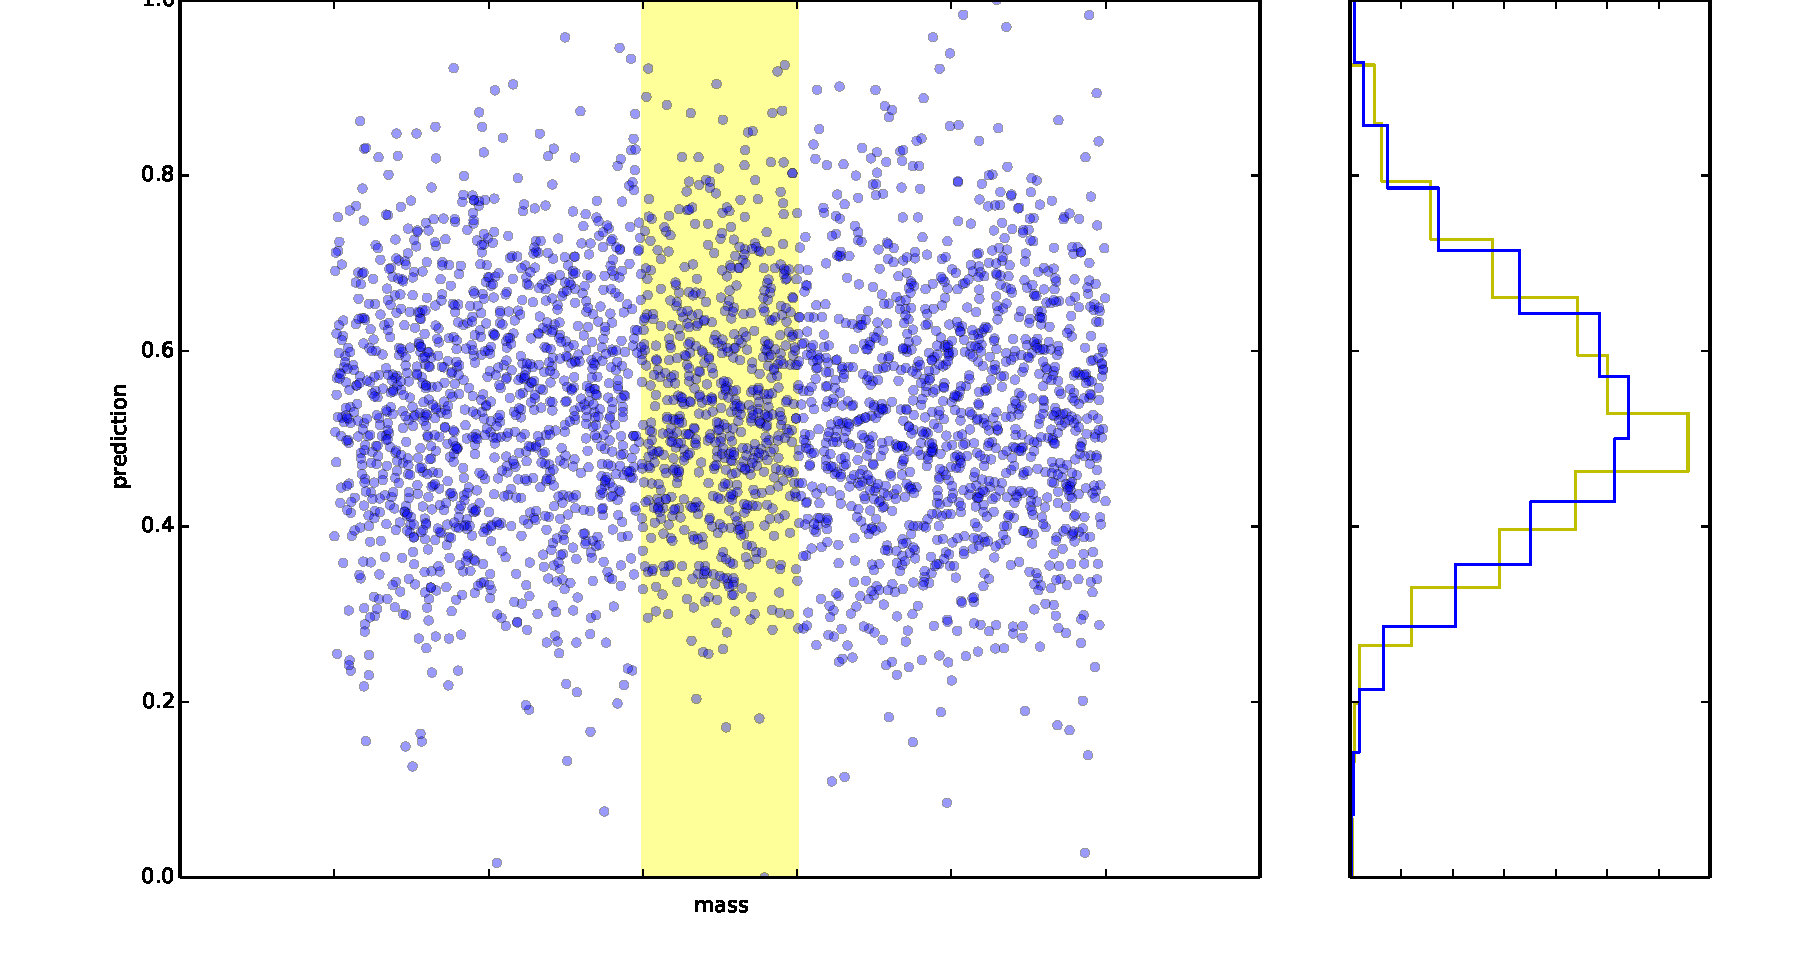
\includegraphics[width=\textwidth]{graphs/bins_uniform_distribution.pdf}
			\caption{Predictions are uniform in mass, the distribution of predictions in the bin (yellow) is close to the global (blue).
			Yellow rectangle shows the events in the bin over mass.}
		\end{subfigure}
		\begin{subfigure}[b]{0.8\textwidth}
			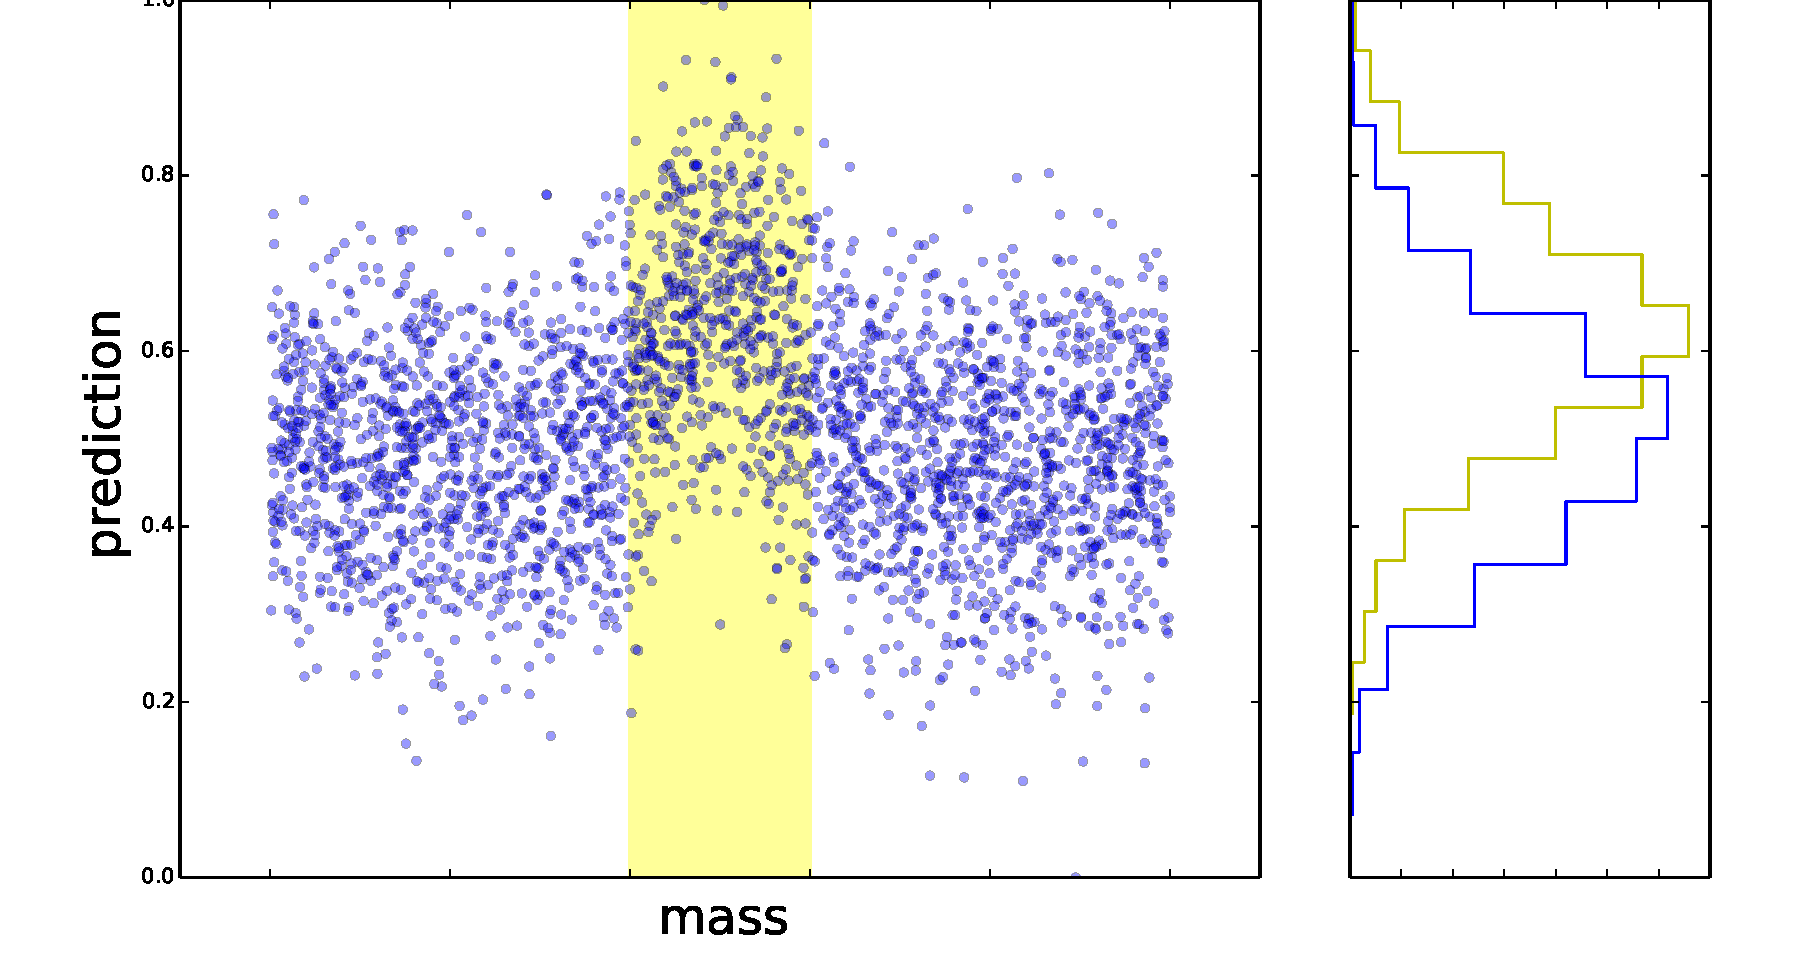
\includegraphics[width=\textwidth]{graphs/bins_nonuniform_distribution.pdf}
			\caption{Distribution with peak in the middle, the distribution in the bin is quite different from global.}
		\end{subfigure}
		\caption{Demonstration of distribution similarity approach. \label{fig:dsavisualization}}
\end{figure}
Instead of measuring uniformity in terms of binned efficiencies, it is possible to consider the distribution of
the binned classifier predictions, $F_\bin$, directly.
Ideal uniformity means that all the distributions $F_\bin$ are equal and hence equal to the global distribution $F(x)$. 
This is demonstrated on figure \ref{fig:dsavisualization}.
To 'measure' non-flatness we can use some distribution distance, like Kolmogorov-Smirnov:
\[
	 \sum_{\bin} \binweight \max_x \abs{F_{\bin}(x) - F(x)},
\]
but Cram\'er--von Mises similarity is more informative (usually $p=2$ is used):
\[
	 \sum_{\bin} \binweight \int \abs{F_{\bin}(x) - F(x)}^p dF(x),
\]
in particular because Kolmogorov-Smirnov measures are too sensitive to local non-uniformities.
The advantage of this method is that we don't need to select some global efficiencies like in the previous metrics.
%\subsection{Connection Between SDE and Distribution Similarity Approach}
%Moreover, SDE and DSA based on Cram\'er--von Mises similarity can be shown to be connected.
%Let's consider the SDE with global efficiencies $= [1/N, 2/N, \dots, N/N]$. In the limit $N \to \infty$
%\[
%	\lim_{N \to \infty} \SDE^2 = 
%	\lim_{N \to \infty} \frac{1}{N} \sum_{\globaleff}\SDE^2(\globaleff) = 
%	\int_0^1 \SDE^2(\globaleff) d\, \globaleff = 
%	\int_0^1 \sum_{\bin} \binweight \abs{\bineff - \globaleff}^2 d\, \globaleff
%\]
%
%From the other side, we can write the expression for similarity-based measure (for $p=2$) 
%\[
%	\sum_{\bin} \binweight \int \abs{F_\text{bin}(x) - F(x)}^2 dF(x) =
%	\int \sum_{\bin} \binweight \abs{F_\text{bin}(x) - F(x)}^2 dF(x) 
%\] The hard thing now is to believe this is literally the same and these two expressions are equal.
%

\subsection{Knn-based modifications}

\def\knni{\text{knn}(i)}
\def\effknni{\text{eff}_{\knni}}
\def\weightknni{\text{weight}_{\knni}}
\def\Fknn{F_{\knni}}

\def\knnSDE{\text{knnSDE}}
\newcommand*\mean[1]{\overline{#1}}


Though operating with bins is usually both simple and very efficient, 
in many cases it is hard to find the optimal size of bins in the space of uniform features (specifically in the case of more than two dimensions).
As mentioned earlier, problems can also arise due to bins with very low populations.

In these cases we can switch to $k$-nearest neighbors: for each signal event we find $k$ nearest signal events (including the event itself)
in the space of uniform features. Now we can compute the efficiency $\effknni$, from the empirical distribution $\Fknn$ of nearest neighbors. 
The weights for $\knni$ are proportional to the total weight of events in $\knni$:
\[
	\weightknni = \alpha \sum_{j \in \knni} w_j, \qquad \alpha^{-1} = \sum_i \sum_{j \in \knni} w_j,
\]
so again weights are normed to 1: $\sum_{i} \weightknni = 1$. 

It is then possible to write the knn versions of SDE
\[
	\knnSDE^2(\globaleff)
		= \sum_{i \in \text{events}} \weightknni \abs{\effknni - \globaleff}^2,
\]
\[
	\knnSDE^2 = \frac{1}{k} \sum_{\globaleff \in [\globaleff_1, \dots \globaleff_k]} \knnSDE^2(\globaleff),
\]
the Theil index of efficiency
\[
	\text{knnTheil}(\globaleff) = \sum_{i \in \text{events}} \weightknni \; \frac{\effknni}{\globaleff} \; \ln{\frac{\effknni}{\globaleff}},
\]
\[
	\text{knnTheil} = \frac{1}{k} \sum_{\globaleff \in [\globaleff_1, \dots \globaleff_k]} \text{knnTheil}(\globaleff),
\]
and the similarity-based measure:
\[
	 \sum_{i \in \text{events}} \weightknni \int \abs{\Fknn(x) - F(x)}^p dF(x).
\]


The knn approach suffers from a drawback: the impact of different events has very little connection with the weights,
because some events are selected as nearest neighbours much more frequently than others.
This effect can be suppressed by dividing the initial weight of the event by the number of times it is selected 
as a nearest neighbour. 

\subsection{Advantages and Disadvantages of Different Metrics}
\subsubsection{Theil and SDE}
Let us compare two metrics that have proven most appropriate for our problem, SDE and Theil. We have some masses distributed uniformly in $[0,1]$, some constant $\alpha$ from interval $[.1,1]$. The predictions are correlated with mass via beta distribution.
We have two distributions that are different in a way that they are symmetrical. SDE should show no changes if we flip the distribution, while the Theil should make difference between pit and peak. 
First distribution with a peak is obtained by generating a prediction for each event according to it mass:
\[
	p \thicksim \text{Beta}(\alpha \mean{m}, \abs{m - \mean{m}})
\]
while the second one has minus sign in front. Figures~\ref{fig:peakdists}~and~\ref{fig:pitdists} show the distribution of the predictions
and classifier efficiency as a function of mass for the peak and pit distributions, respectively. 
\begin{figure}[h]
\centering
		\begin{subfigure}[b]{0.95\textwidth}
			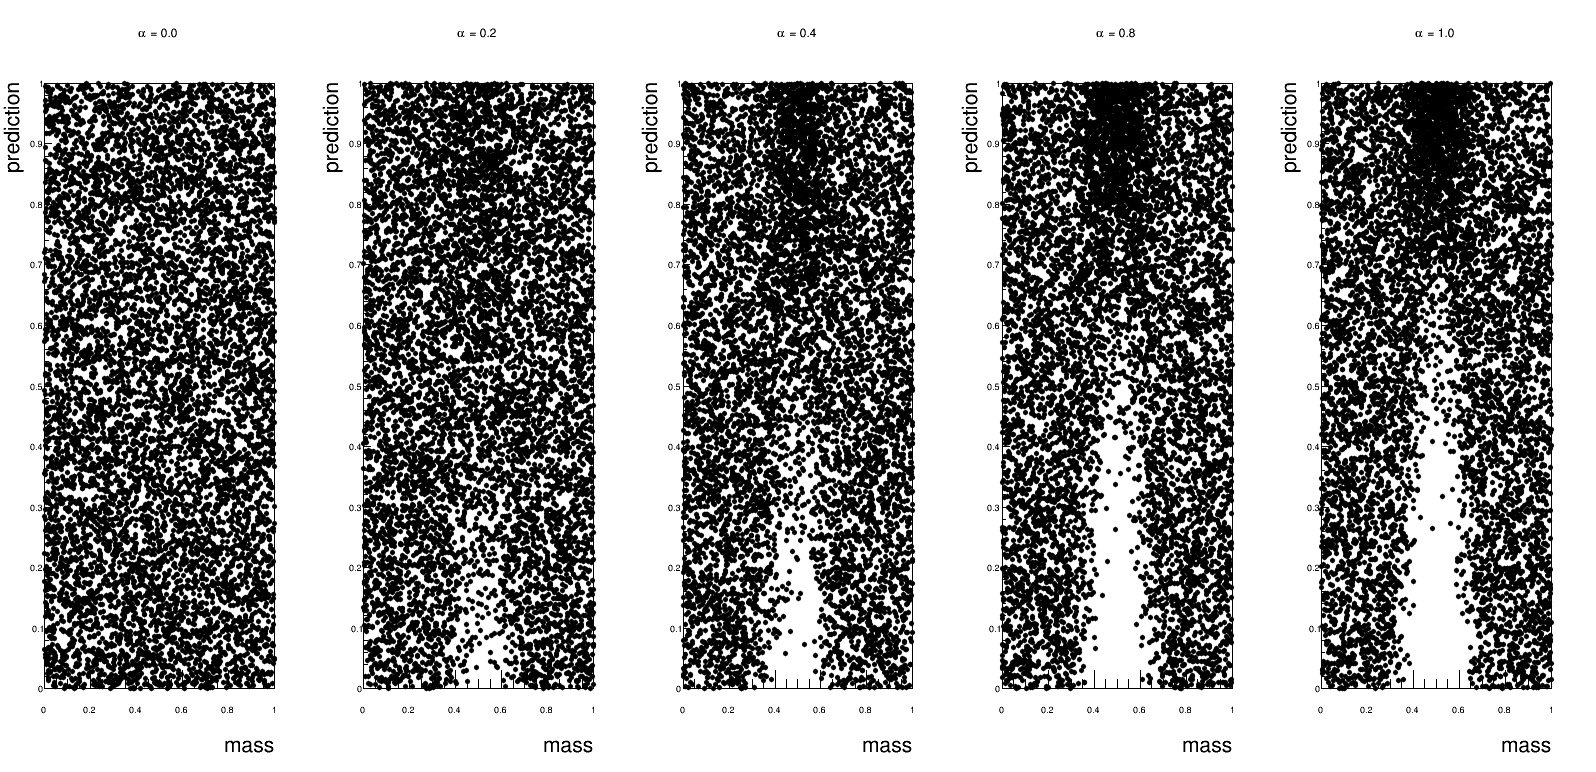
\includegraphics[width=\textwidth]{graphs/PeakDistributions.png}
			\caption{Mass vs prediction.}
		\end{subfigure}
		\begin{subfigure}[b]{0.95\textwidth}
			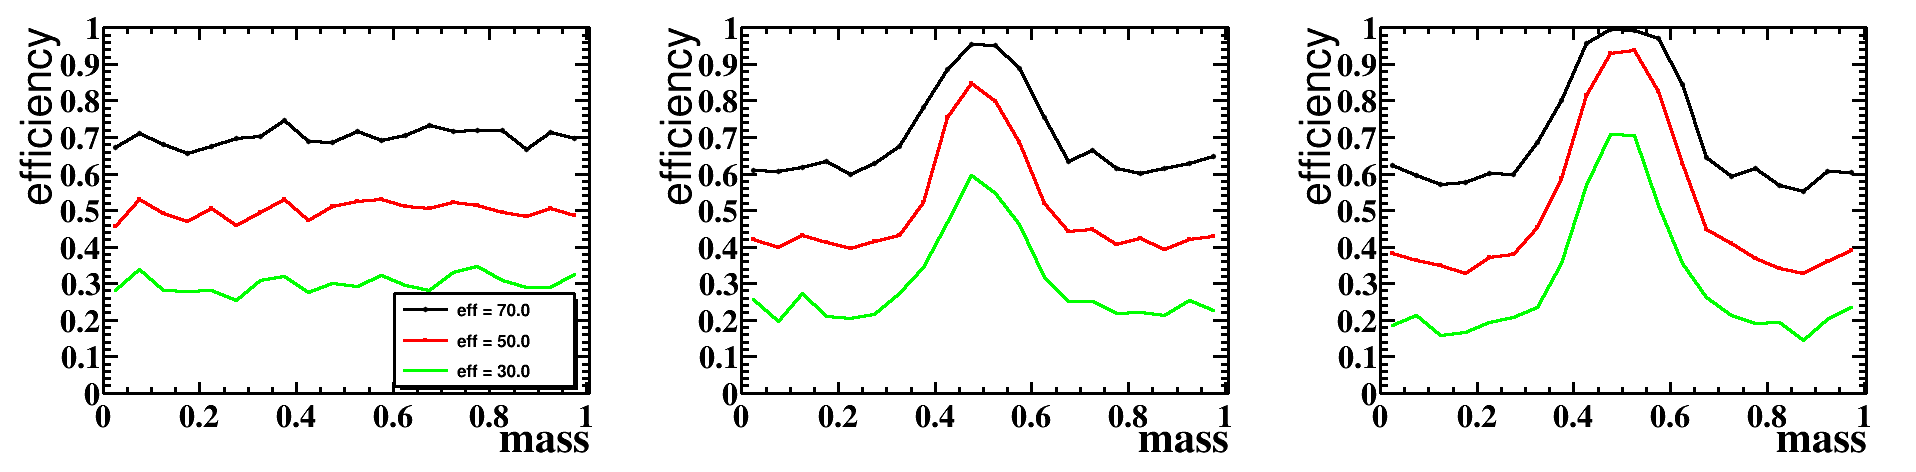
\includegraphics[width=\textwidth]{graphs/PeakEffs.png}
			\caption{Mass vs efficiency. The different coloured lines correspond to
				different global classifier efficiencies, as explained in the legend on the leftmost subplot.}
		\end{subfigure}
		\caption{Peak response distribution and efficiencies as a function of mass. \label{fig:peakdists}}
\end{figure}

\begin{figure}[h]
\centering
		\begin{subfigure}[b]{0.95\textwidth}
			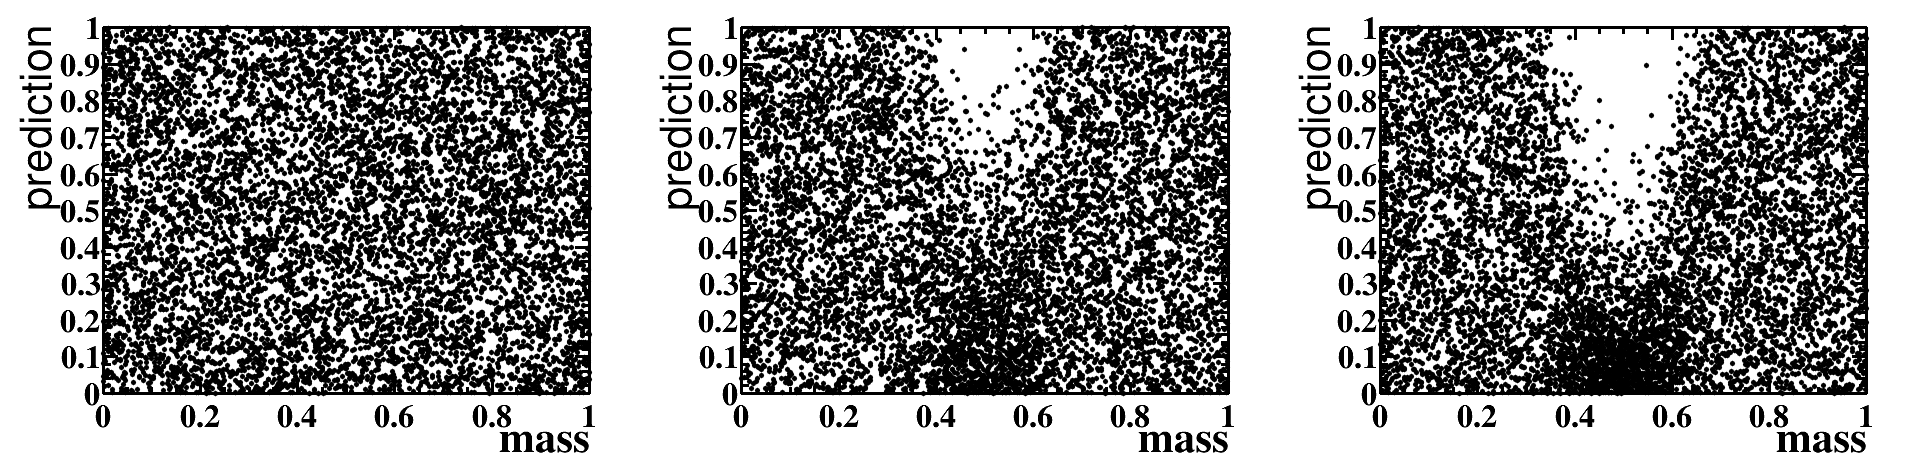
\includegraphics[width=\textwidth]{graphs/PitDistributions.png}
			\caption{Mass vs prediction.}
		\end{subfigure}
		\begin{subfigure}[b]{0.95\textwidth}
			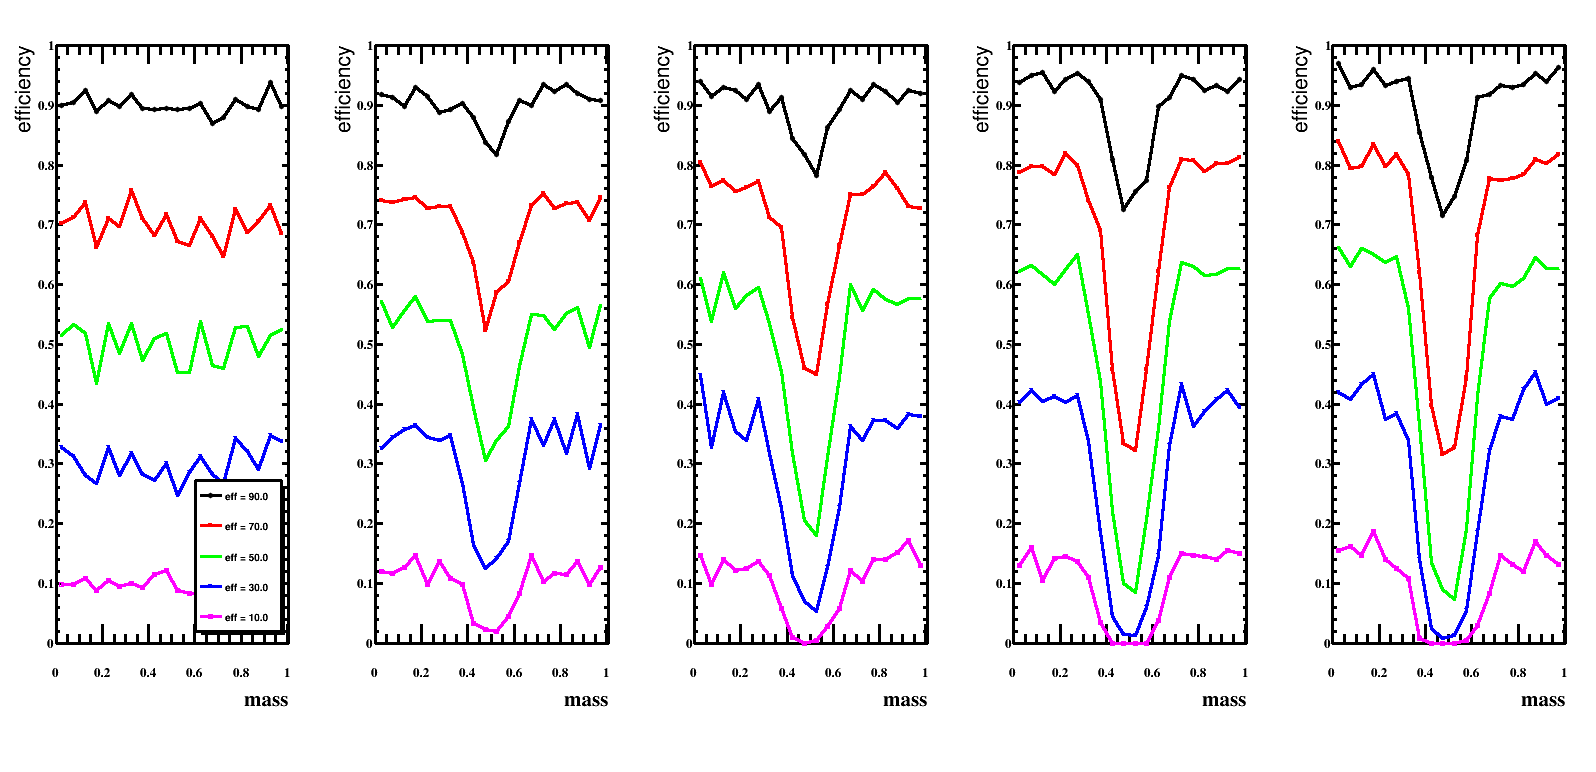
\includegraphics[width=\textwidth]{graphs/PitEffs.png}
			\caption{Mass vs efficiency. The different coloured lines correspond to
				different global classifier efficiencies, as explained in the legend on the leftmost subplot.}
		\end{subfigure}
		\caption{Pit response distribution and efficiencies as a function of mass. \label{fig:pitdists}}
\end{figure}

\begin{figure}[h]
\centering
	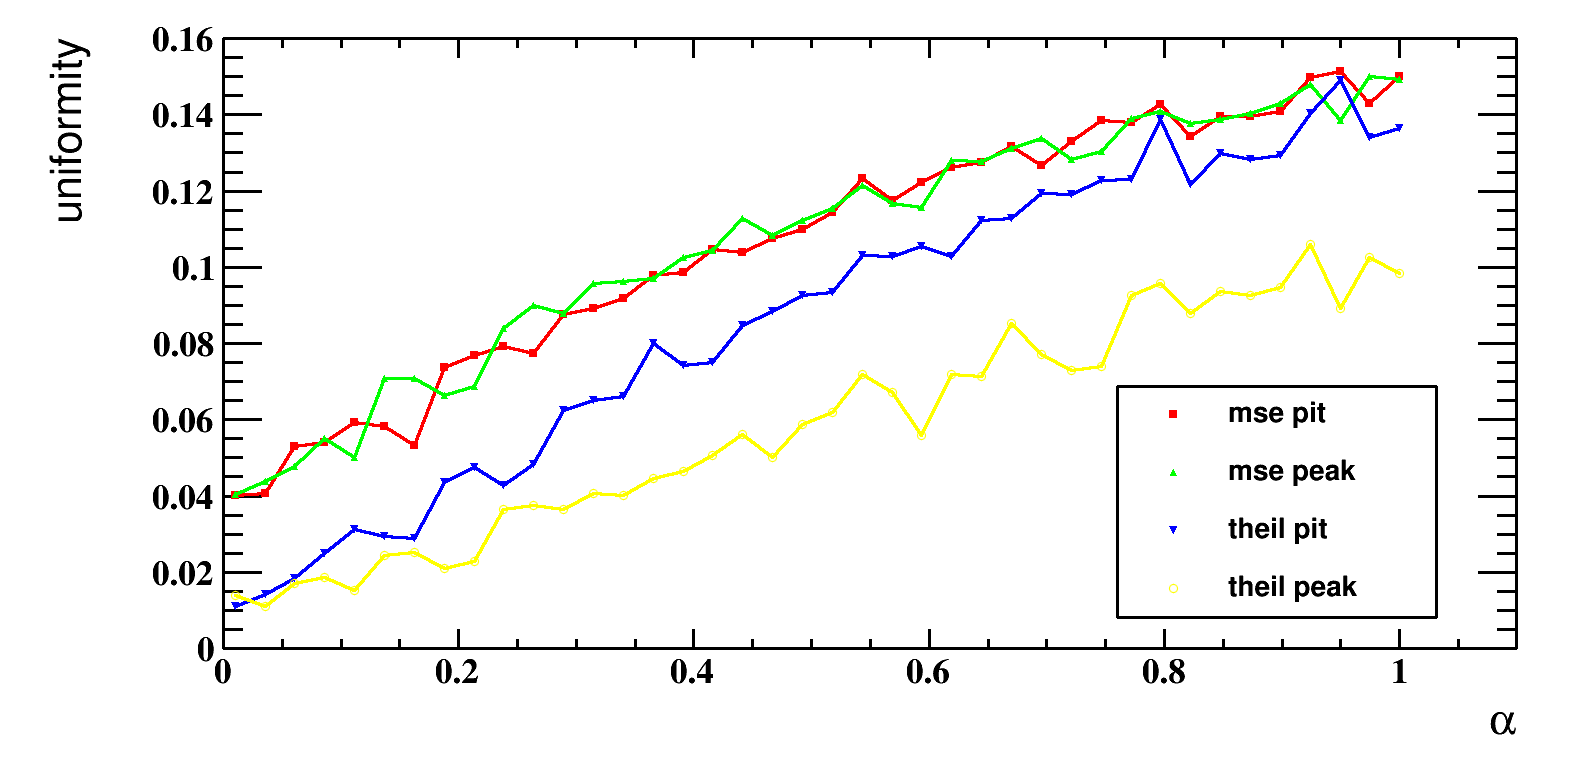
\includegraphics[width=0.5\textwidth]{graphs/TheilVsMSE.png}
	\caption{Comparison of SDE and Theil uniformity measures for different values of the constant $\alpha$ for the peak and pit distributions.
The Theil can clearly distinguish between these two while the SDE measure cannot.}
\end{figure}

From these figures we can see that SDE has the same value and it is not able to make difference between these distributions. In the second case Theil has lower value which indicates that distribution is flatter. In the combination with SDE it can be used to detarmine the type of a distribution. Lower value of SDE can indicate that distribution is flat or has some narrow peaks or pits, and by using Theil we can distinguish between these two cases.

\subsubsection{$D \to hhh$}
When our classifiers where applied to data set $D \to hhh$ we got uniformity measures for the SDE and Theil
metrics shown in Fig.~\ref{fig:d2hhhsdetheil}.
\begin{figure}[h]
\centering
		\begin{subfigure}[b]{0.95\textwidth}
			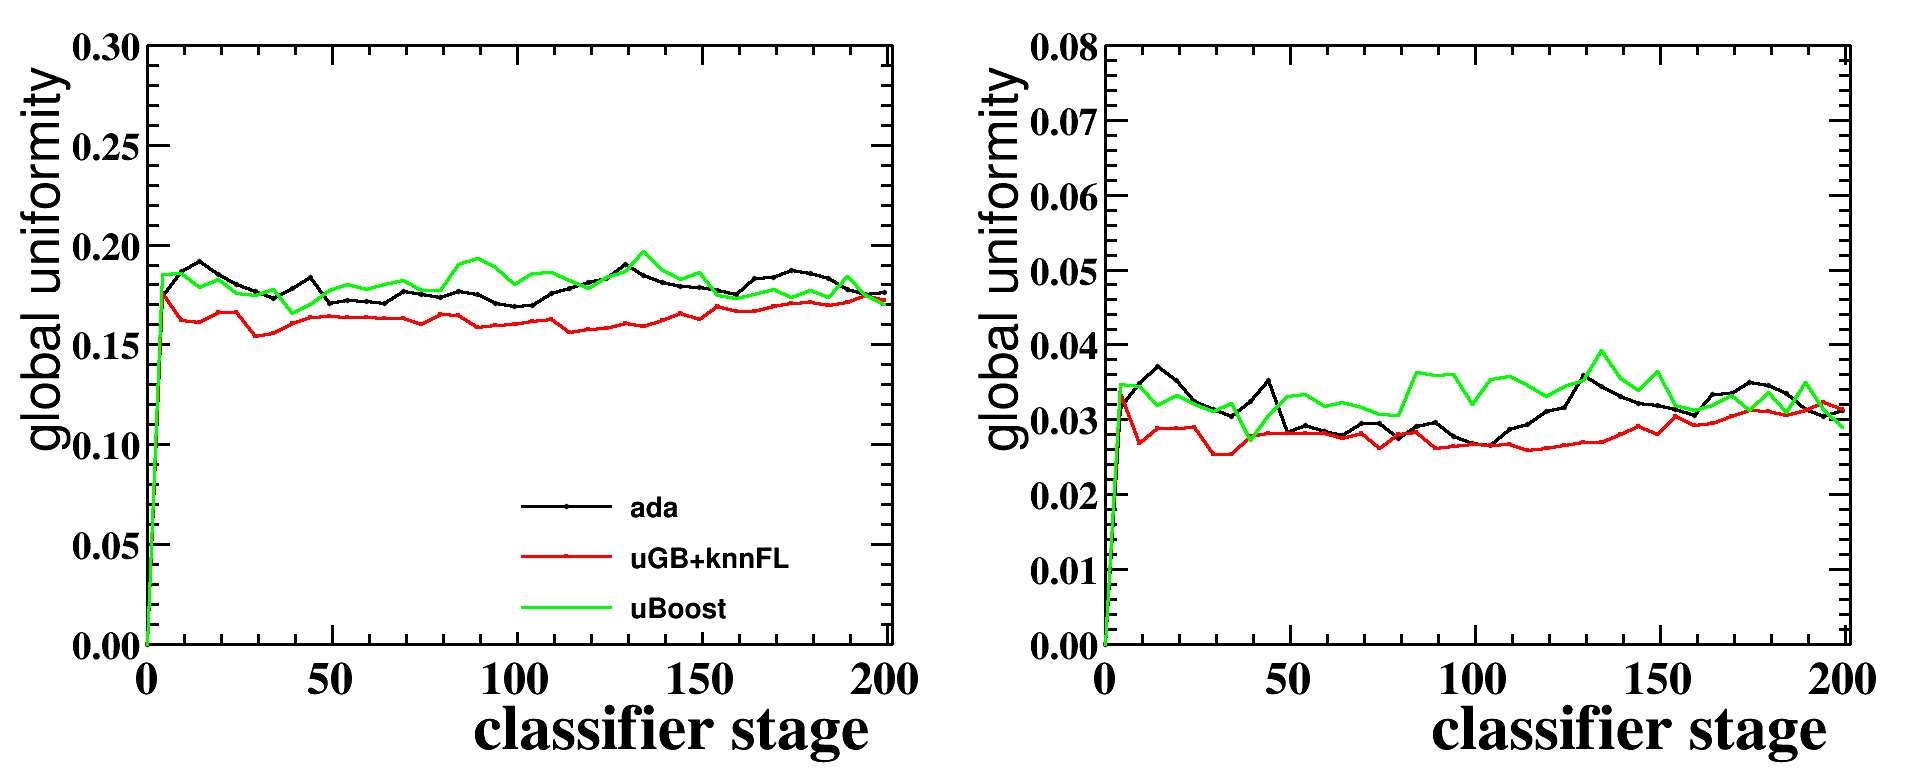
\includegraphics[width=\textwidth]{graphs/D23hSignalEffs.png}
			\caption{Metrics for $D \to hhh$ signal.}
		\end{subfigure}
		\begin{subfigure}[b]{0.95\textwidth}
			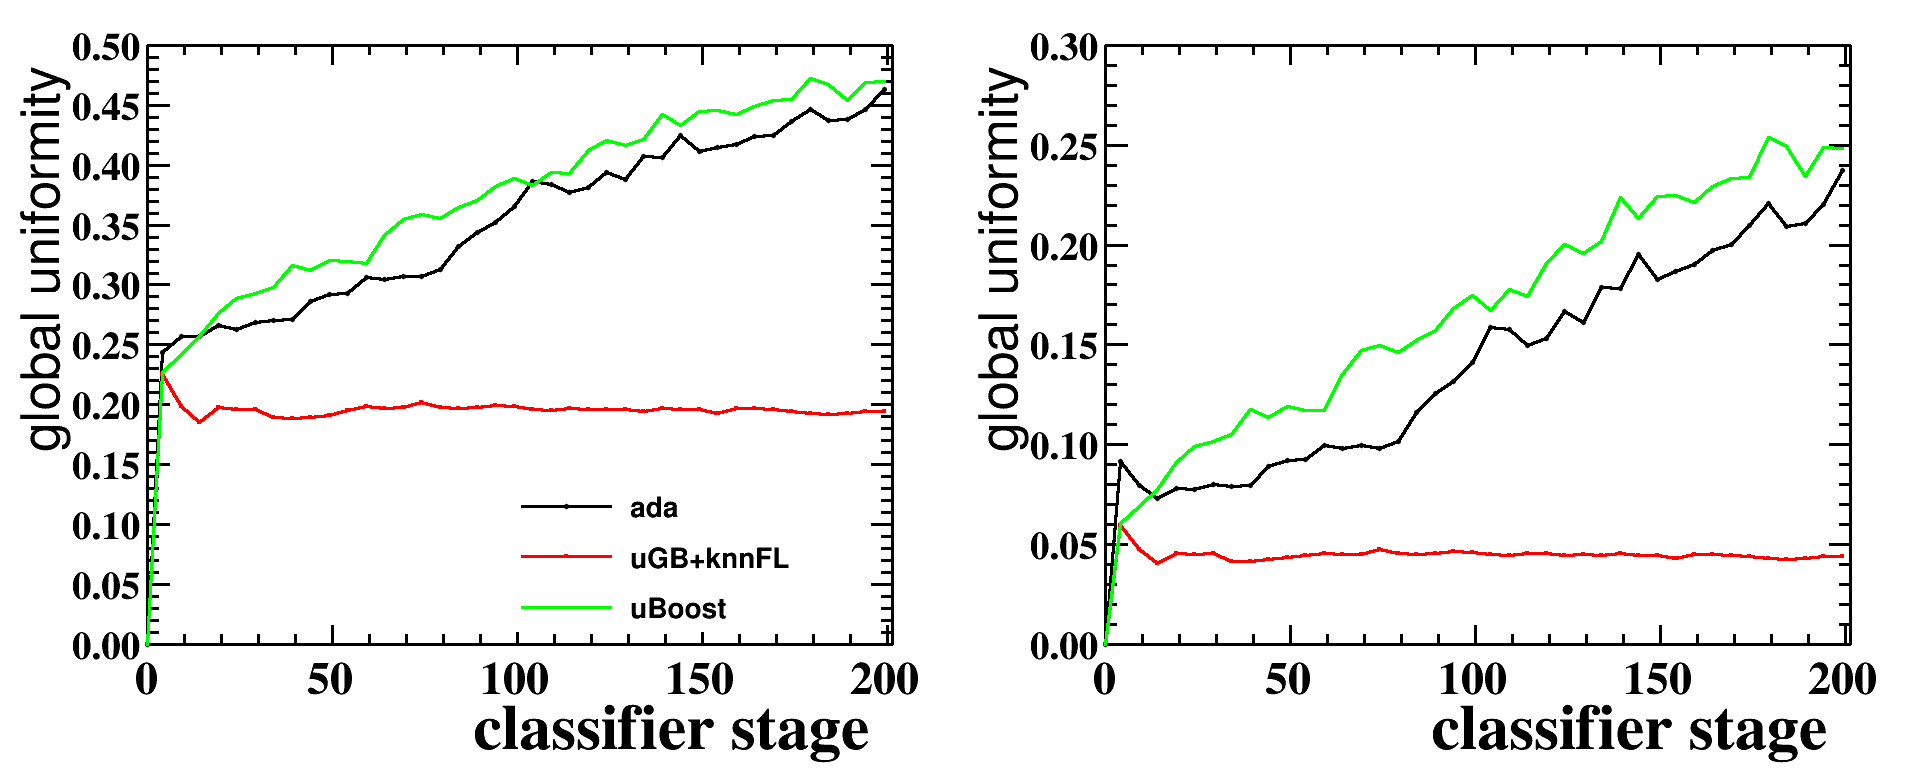
\includegraphics[width=\textwidth]{graphs/D23hBgEffs.png}
			\caption{Metrics for $D \to hhh$ background.}
		\end{subfigure}
		\caption{Uniformity metrics for the $D \to hhh$ data set. The (top) signal and (bottom) background uniformities are plotted as a function of the training stage of a given classifier, listed in the legends on the leftmost plots. \label{fig:d2hhhsdetheil}}
\end{figure}

Both metrics shown similar results, and that there is no significant difference on real data sets (as well as CvM).
The SDE and Theil metrics can be used together in limit cases to more precisely determine nature of a distribution.


\section{Approaches Proposed}

\section{Boosting approaches}
\subsection{Mean Ada Boost}

This is a modification of AdaBoost algorithm. In AdaBoost one multiplies weights in such a way:
\[
	w_i = w_i \times \exp[-y_i \, \text{score}_i],
\]
to enlarge the weights of poorly classified events ($y_i$ is $+1$ for signal and $-1$ for background).

But now we use the mean of prediction of $k$ nearest neighbors (of the same class)
\[
	w_i = w_i \times \exp[-y_i \, \dfrac{1}{k} \sum_{j \in \knni} \text{score}_j]
\]
Thus boosting focuses not on the events that were poorly classified, but on the regions with poor classification.


\subsection{Gradient Boosting with AdaLoss Modification (knn-Ada)}

\def\score{\text{score}}
\def\knn{\text{knn}}
\def\FL{\text{FL}}

Gradient boosting on trees is widely used algorithm[link], it's built upon decision tree regressors with usage of some loss function. 

Let's start with examples. One of the popular losses used is AdaLoss:
\[
	\sum_{i \in \text{events}} w_i \times \exp [- \score_i \, y_i] 
\]
where $y_i$ is either +1 (for signal events) or -1 (for background events). Good classification supposes that signal events should have large positive scores, while background ones should have large negative.

The predictions of separate regressors are simply summed up to form a score:
\[
	\score_i = \sum_{r \in \text{regressors}} \text{pred}_r(i),
\]
which can be 'translated' into probabilities by logistic function.

So the goal of algorithm is now to minimize the loss function. At each stage it trains one more regressor, which should decrease the value of loss, the most vivid way is to train it on negative gradient of loss. In the case of AdaLoss this can be done pretty easy:
\[
	-\dfrac{\partial \, \text{AdaLoss}}{\partial \, \score_i} = w_i \, y_i \exp[- \score_i \, y_i],
\]
so it is positive for signal events, negative for background events and has larger modulus for the events which are poorly classified.


This loss function can be easily modified to take in account not only the score for individual elements, but also 'finds' regions with lower-than-average quality.

\[
	\text{knnAdaLoss} = \sum_{i \in events} \exp[-y_i \times \sum_{j \in \text{knn}(i)} \score_j],
\]
where the index $j$ goes over the $k$ nearest neighbors of $i$th event, which belongs to the same class (signal or background).

We can introduce a supplementary sparse matrix $A \in \RR^{N \times N}$ ($N$ is number of events), which is defined as 
\[
a_{ij} = \begin{cases} 
1, & j \in \knn(i), \text{ events $i$ and $j$ belong to the same class} \\
0, & \text{otherwise},
\end{cases}
\] so the loss can be written as
\[
	\text{knnAdaLoss} = \sum_i \exp [- y_i \sum_j a_{ij} \, \score_j ],
\]
it's negative gradient is easily computed:
\[
	-\dfrac{\partial \, \text{knnAdaLoss}} {\partial \, \score_k} = 
	 y_k \, \sum_i a_{ik} \exp [- y_i \sum_j a_{ij} \, \score_j ],
\]
from this we can see that new algorithm will pay more attention to the events, which has poorly classified neighbors (and neighbors of neighbors). The named loss targets to obtain uniformity in both signal and background.

One can note, that the matrix $A$ doesn't need to be necessarily square. One can introduce $M$ groups of events (which may intersect), each group consists of several events with close uniform variables (and close events). Then one introduces $A \in \RR^{M \times N}$:
\[
	a_{mj} = \begin{cases}
		1, & \text{event $j$ is in group $m$} \\
		0, & \text{otherwise}
	\end{cases}
\]

In particular, if we take $A$ to be identity matrix: $A = I$ (each event to be in it's own group), knnAdaLoss turns into a simple AdaLoss.



\subsection{Gradient Boosting with Flatness Loss (FL)}

Let's use the metrics introduces in the section \ref{sec:similarity}:
\[
	\sum_{\bin} \binweight \int \abs{F_{\bin}(x) - F(x)}^p dF(x),
\]
which is good as a measure, but due to the non-smoothness of $F(x)$ it's 
gradient is singular, so we use instead
\[
	\FL = \sum_{\bin} \binweight \int \abs{F_{\bin}(x) - F(x)}^p dx.
\]

So, the derivative looks like:
\[
	\dfrac{\partial} {\partial \, \score_i} \FL
	= \sum_{\bin} \binweight \frac{\partial }{ \partial \, \score_i} 
			\int \abs{F_\bin(x) - F(x)}^p dx
\]
Let $\bin(i)$ be a bin to which event $i$ belongs, then we can compute:
\def\binIweight{\text{weight}_\text{\bin(i)}}


\begin{multline*}
	- \dfrac{\partial} {\partial \, \score_i} \FL = 
		- \binIweight
		\frac{\partial }{ \partial \, \score_i} 
			\int \abs{F_{\bin(i)}(x) - F(x)}^p dx \cong \\
	\cong \binIweight \, p \,  \abs{F_{\bin(i)}(x) - F(x)}^{p-1} 
		\sgn[F_{\bin(i)}(x) - F(x)]
		\dfrac{w_i}{\binIweight}
		\Bigg|_{x=\score_i} = \\
	= 
		w_i \, p \,  \abs{F_{\bin(i)}(x) - F(x)}^{p-1}
		\sgn[F_{\bin(i)}(x) - F(x)]
		\Bigg|_{x=\score_i}
\end{multline*}

Explanation:
\begin{multline*}
	- \dfrac{\partial} {\partial \, \score_i} \FL = 
		- \binIweight \frac{\partial }{ \partial \, \score_i} \int \abs{F_{\bin(i)}(x) - F(x)}^p dx = \\
	= \binIweight \abs{F_{\bin(i)}(x) - F(x)}^p \bigg|_{x=\score_i-}^{x=\score_i+} = \\
	= \{ \text{assuming that $F_{\bin(i)}(x)$, $F(x)$ changed small } \} = \\
	= \binIweight p \abs{F_{\bin(i)}(x) - F(x)}^{p-1} \sgn(F_{\bin(i)}(x) - F(x)) \left[F(x-) - F(x+) + F_{\bin(i)}(x+) - F_{\bin(i)}(x-)\right] \bigg|_{x=\score_i}= \\
	= \binIweight p \abs{F_{\bin(i)}(x) - F(x)}^{p-1} \sgn(F_{\bin(i)}(x) - F(x)) \left[- \frac{w_i}{\sum_j w_j} + \frac{w_i}{\binIweight} \right] \bigg|_{x=\score_i}= \\
	= \{ \text{ignoring $\frac{w_i}{\sum_j w_j}$}  \}
	\cong \binIweight \, p \,  \abs{F_{\bin(i)}(x) - F(x)}^{p-1} 
	% 	\sgn[F_{\bin(i)}(x) - F(x)]
	% 	\dfrac{w_i}{\binIweight}
	% 	\Bigg|_{x=\score_i} = \\
	% = 
	% 	w_i \, p \,  \abs{F_{\bin(i)}(x) - F(x)}^{p-1}
	% 	\sgn[F_{\bin(i)}(x) - F(x)]
	% 	\Bigg|_{x=\score_i}
\end{multline*}


The next thing we need to point is FL doesn't take into account the quality of predictions. So what we use in practice is linear combination of FlatnessLoss and AdaLoss:
\[
	\text{loss} = \FL + \alpha \, \text{AdaLoss}
\]

First one penalizes the non-uniformity, second one --- poor predictions.


\section{Dataset}

\section{Datasets}
This study uses simulated event samples produced using the official LHCb simulation framework.
The software used for the generation of the events is described in LHCb publications as follows :

\begin{quote}
In the simulation, $pp$ collisions are generated using
PYTHIA~\cite{Sjostrand:2006za} 
with a specific LHCb configuration~\cite{LHCb-PROC-2010-056}.  Decays of hadronic particles
are described by EvtGen~\cite{Lange:2001uf}, in which final state
radiation is generated using PHOTOS~\cite{Golonka:2005pn}. The
interaction of the generated particles with the detector and its
response are implemented using the GEANT
toolkit~\cite{Allison:2006ve, Agostinelli:2002hh} as described in
Ref.~\cite{LHCb-PROC-2011-006}.
\end{quote}

All simulated event samples are generated inside the LHCb detector acceptance.
The signal used in this analysis consists of $D_s^\pm\to\pi^+\pi^-\pi^\pm$ decays, simulated
using the $\textrm{D}\_\textrm{DALITZ}$ model of EvtGen to simulate the intermediate resonances which contribute to the
three pion final state. The background candidates are three pion combinations reconstructed in
simulated samples of $c\bar{c}$ and $b\bar{b}$ events, where the charm and bottom quark decays are
inclusively modelled by EvtGen. The simulated events contain ``truth'' information which identifies them as
signal or background, and which identifies the physical origin of the three pion combinations reconstructed
in the $c\bar{c}$ and $b\bar{b}$ simulated samples.


\section{Plots}

\input{parts/plots}

\section{Timings}

The main drawback of uBoost technique is it's high computational complexity: 
while simple AdaBoost trains $M$ trees, uBoost builds $100 \times M$ trees (contribution of other operations usually can be neglected). 

Presented in this paper classifiers are building $M$ trees, though there is more complicated boosting, it takes at each iteration ($k$ is number of neighbors, $N$ is number of events in training sample)

\begin{itemize}
	\item meanAdaBoost: $O(k \times N)$
	\item knnAdaLoss: $O(k \times N)$, for the arbitrary matrix $A$ it is 
	$O( \text{\#nonzero elements in the matrix})$
	\item FlatnessLoss: $O(N \ln N)$
\end{itemize}


\section{Summary}

A number of novel boosting algorithms have been presented that consider uniformity of selection efficiency in a multivariate space in addtion to misclassifcation errors.  Of these, the UGBFL algorithm has the best performance on the example analyses studied in this paper.
This algorithm is expected to be useful in a wide-variety of analyses performed in particle physics.


\section{Source code}

The link on the repository ans links to final notebooks with results in the article.

\acknowledgments

These results were obtained using events generated with the official LHCb simulation, and we are grateful to the LHCb collaboration for this privilege. 
We particularly acknowledge the work of the LHCb Simulation and Core Computing teams in tuning the simulation software and managing the productions of simulated events.

\begin{thebibliography}{9}

\bibitem{Sjostrand:2006za}
{"Sj\"{o}strand, Torbj\"{o}rn and Mrenna, Stephen and Skands, Peter"},
\emph{PYTHIA 6.4 physics and manual},
\href{http://dx.doi.org/10.1088/1126-6708/2006/05/026},
{\emph{JHEP} {\bf 05} (2006) 026},
[\hepph{0603175}].

\bibitem{LHCb-PROC-2010-056}
{"Belyaev, I. and others"},
\emph{Handling of the generation of primary events in GAUSS, the LHCb simulation framework},
\href{http://dx.doi.org/10.1109/NSSMIC.2010.5873949},
{\emph{NSS/MIC} {\bf IEEE} (2010) 1155}.

\bibitem{Lange:2001uf}
{"Lange, D. J."},
\emph{The EvtGen particle decay simulation package},
\href{http://dx.doi.org/10.1016/S0168-9002(01)00089-4},
{\emph{NIM} {\bf A462} (2001) 152-155}.

\bibitem{Golonka:2005pn}
{"Golonka, Piotr and Was, Zbigniew"},
\emph{PHOTOS Monte Carlo: a precision tool for QED corrections in $Z$ and $W$ decays},
\href{http://dx.doi.org/10.1140/epjc/s2005-02396-4},
{\emph{EPJ} {\bf C45} (2006) 97-107},
[\hepph{0506026}].

\bibitem{Allison:2006ve}
{"Allison, John and Amako, K. and Apostolakis, J. and Araujo, H. and Dubois, P.A. and others"},
\emph{Geant4 developments and applications},
\href{http://dx.doi.org/10.1109/TNS.2006.869826},
{\emph{IEEE TNS} {\bf 53} (2006) 270}.

\bibitem{Agostinelli:2002hh}
{"Agostinelli, S. and others"},
\emph{Geant4: a simulation toolkit},
\href{http://dx.doi.org/10.1016/S0168-9002(03)01368-8},
{\emph{NIM} {\bf A506} (2003) 250}.

\bibitem{LHCb-PROC-2011-006}
{"Clemencic, M and others"},
\emph{The LHCb simulation application, GAUSS : design, evolution and experience},
\href{http://dx.doi.org/10.1088/1742-6596/331/3/032023},
{\emph{J. Phys. Conf. Ser.} {\bf 331} (2011) 032023}.

% The examples of items:
% \bibitem{bib1}
% Authors,
% \emph{Title},
% \emph{J. Ref.} \textbf{vol} (year) page.

% \bibitem{bib2}
% A. Pietropaolo et al., \emph{DINS measurements on VESUVIO in the
%     resonance detector configuration: proton mean kinetic energy in
%     water}, \jinst{1}{2006}{P04001}.

% \bibitem{bib3}
% A.I. Harris,
% \emph{Spectroscopy with multichannel correlation radiometers},
% \href{http://dx.doi.org/10.1063/1.1898643}
% {\emph{Rev.\ Sci.\ Instrum.} {\bf 76} (2005) 054503}
% [\astroph{0504449}].

% \bibitem{bib4}
% G.F. Knoll, \emph{Radiation detection and measurements}, John Wiley
%     and Sons, Inc., New York 2000.

% \bibitem{bib5}
% V. Dangendorf, \emph{Time-resolved fast-neutron imaging with a
% pulse-counting image intensifier}, in proceedings of
% \emph{International workshop on fast neutron detectors and
% applications}, April, 3--6, 2006 University of Cape Town, South Africa
% \pos{PoS(FNDA2006)008}.

\end{thebibliography}

\end{document}
